\chapter{Classification Approaches}
\label{cap:classification_approaches}
The following chapter describes the general architecture of existing classifiers, presents models selected as references to the proposed solution, and adjustments made to these models to make them fit the task of on-line speech and music classification.

\section{Overview}

\begin{figure}[htbp]
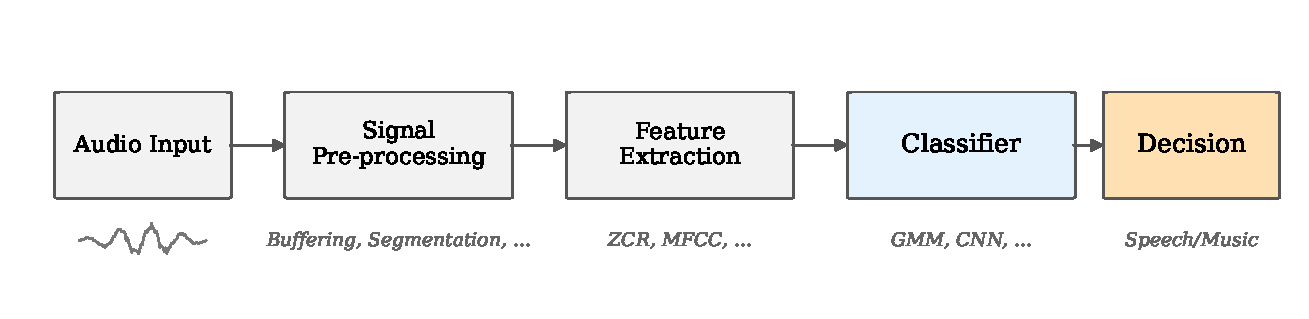
\includegraphics[width=\textwidth]{figures/general_classifier.pdf}
\label{fig:general_classifier}
\caption{Example diagram of generic speech/music classifier}
\end{figure}

Classifiers are algorithms whose goal is to assign an input sample to one of a set of predefined classes.

Figure~\ref{fig:general_classifier} illustrates a minimal processing pipeline of a generic classification system.

The first stage of the pipeline consists of pre-processing steps, which are largely influenced by the architecture of specific classifier and its application.
In the case of on-line audio classification, buffering and segmentation of the input signal are required due to the constraints described in \cref{subsec:constraints}.

Raw input samples do not provide a robust representation of an audio signal, which motivates the use of feature extraction in the majority of audio classification pipelines.

Although a speech and music classifier can operate as a standalone application, audio classifiers are most commonly used as pre-processing components in larger processing pipelines.
As a module in this context, classifiers often serve to prevent subsequent processing stages from wasting computational resources or from operating on inactive or invalid input.

\section{Traditional Methods}
Traditional methods of speech and music classification refer to usage of machine learning algorithms such as Gaussian Mixture Models, Decision Trees or Support Vector Machines.

The advantage of using machine learning models in comparison to deep learning algorithms is the low computational complexity in both training and inference stages.

Main drawback of traditional methods is the need for selection of right features to represent input signal as they cannot work on raw input.
Selection is carried out by thorough experiments with combinations of features or integration of the selection algorithm, such as sequential forward/backward floating selection~\cite{PUDIL19941119}, for the selection of best features by eliminating features with low variance.

\section{Reference Machine Learning Models}
Models in this subsection were picked as references to the proposed method.

\subsection{Decision Tree Classifier by Lavner and Ruinskiy~\cite{Lavner2009-zo}}
This method proposed a decision-tree-based algorithm for speech and music classification.

Feature extraction and selection for this model is implemented as described by the paper.
Authors assume every input segment is either speech or music; silent and noisy frames must therefore be eliminated from the training phase of the model.
For the fairness of comparison, all models were evaluated on 2-class and 3-class classification task.

\textcolor{green}{separate tables?}

\subsection{Gaussian Mixture Model and Support Vector Machine by Khonglah and Prasanna~\cite{KHONGLAH201671}}

This method proposes two classifiers — a Gaussian Mixture Model (GMM) and a Support Vector Machine (SVM) — sharing the same feature extraction pipeline.

\subsubsection*{Feature Extraction}
Audio is processed at 16\,kHz with 30\,ms frames and a 15\,ms hop.
A 1-second rolling buffer accumulates per-frame features to compute long-term statistics.

The feature vector contains the following per-frame features: short-time energy, zero-crossing rate (ZCR), spectrum centroid, spectral flux, and spectral rolloff point (85th percentile).
Over the 1-second buffer, the variance of ZCR, spectrum centroid, spectral flux, and rolloff are computed, together with the Low Short-Time Energy Ratio (LSTER).

Additionally, speech-specific features are computed at 1\,ms resolution within a secondary buffer: the normalized autocorrelation peak strength of the zero-frequency filtered signal (NAPS of ZFFs), the peak-to-sidelobe ratio of the Hilbert envelope of the LP residual (PSR-HE), log mel-spectrum energy (22 Mel bands, 0–4\,kHz), and modulation spectrum energy in the syllabic band (2–10\,Hz).
Per-feature means of the secondary buffer are appended to the feature vector.

\subsubsection*{Gaussian Mixture Model}
Two GMMs — one for speech and one for music — are trained on features scaled with a \texttt{RobustScaler}.
Each GMM has 8 components with diagonal covariance, $k$-means initialization, and a regularization term of $10^{-4}$ added to the covariance diagonals.

At inference, the log-likelihood delta $\delta = \log p_{\text{speech}}(\mathbf{x}) - \log p_{\text{music}}(\mathbf{x})$ is computed per frame and accumulated in a 66-frame rolling buffer (approximately 1\,s at 15\,ms hop).
The smoothed mean of the buffer determines the prediction: speech if $\bar{\delta} > 0$, music otherwise.

\subsubsection*{Support Vector Machine}
The SVM uses an RBF kernel with $C = 1$ and $\gamma = 3$, matching the paper, and operates within a \texttt{StandardScaler} pipeline.
Only speech and music frames participate in training; noise frames are excluded.
The training set is randomly subsampled to at most 50\,000 frames per class to keep training tractable at the frame level.

At inference, the raw SVM decision function values are accumulated in a 20-frame rolling buffer.
The smoothed mean determines the label: speech if negative, music otherwise.

Unlike the GMM, the SVM does not natively produce calibrated probabilities; evaluation therefore relies on the hard decision output.

\subsubsection*{Differences from the Paper}
The paper trained on approximately 160 audio clips represented as 1-second non-overlapping window vectors, whereas this implementation trains on frame-level features with per-class subsampling.
Feature scaling uses \texttt{RobustScaler} for the GMM and \texttt{StandardScaler} for the SVM, rather than per-clip log-mel normalization as in the original.
The sigmoid mapping on the log-likelihood delta described in the paper is not applied; smoothing is performed directly on the raw delta.
Neither model handles the inactive (noise) class — both output only speech or music — resulting in zero F1 for inactive segments in the 3-class evaluation.

\subsubsection*{Results}

Table~\ref{tab:gmm_svm_results} shows per-class and macro F1, precision, and recall on the 2-class evaluation.
In the 3-class evaluation, both models predict only speech or music, leaving inactive segments entirely misclassified; macro F1 drops to 0.5552 for the GMM and 0.5489 for the SVM.

\begin{table}[h]
\centering
\begin{tabular}{llccc}
\hline
Model & Class & F1 & Precision & Recall \\
\hline
\multirow{3}{*}{GMM} & Speech  & 0.8351 & 0.7775 & 0.9018 \\
                     & Music   & 0.8445 & 0.9078 & 0.7894 \\
                     & \textbf{Macro}   & \textbf{0.8398} & 0.8427 & 0.8456 \\
\hline
\multirow{3}{*}{SVM} & Speech  & 0.8088 & 0.8297 & 0.7889 \\
                     & Music   & 0.8508 & 0.8344 & 0.8679 \\
                     & \textbf{Macro}   & \textbf{0.8298} & 0.8321 & 0.8284 \\
\hline
\end{tabular}
\caption{2-class evaluation results for GMM and SVM on the test split.}
\label{tab:gmm_svm_results}
\end{table}

The GMM achieves higher recall for speech (0.9018 vs.\ 0.7889) while the SVM is more balanced.
Average inference time per frame is 4.9\,ms for the GMM and 6.6\,ms for the SVM.

\section{Deep Learning Methods}

\section{Reference Deep Learning Models}

\subsection{YamNET~\cite{drossos2020soundeventdetectiondepthwise}}


%Most classifiers do not operate directly on raw input samples, as these typically do not provide a compact or robust representation of the signal characteristics.
%Instead, a feature extraction stage is employed to transform the buffered audio segments into a set of descriptive features that capture relevant temporal and spectral properties of the signal.
%Commonly used features in speech and music classification include spectral features, energy-based measures, and statistics computed over short time windows.

%The extracted features are then passed to the classification model, which maps the feature representation to one of the predefined classes.
%Various model architectures can be used at this stage, ranging from traditional machine learning approaches to modern neural network-based methods.
%The choice of the classification model is influenced by factors such as classification accuracy, computational complexity, and suitability for on-line operation.

%Finally, the classifier output may be post-processed to obtain more stable decisions over time.
%This step can include temporal smoothing or aggregation of multiple frame-level decisions into a single segment-level output.
%In speech and music classification, the final result is typically a binary decision indicating whether the input signal corresponds to speech or music.
